\documentclass[a4paper, 12pt]{article}

\usepackage{mathtools}
\usepackage{graphicx}
\usepackage{amsmath}

\usepackage{caption}
\usepackage{subcaption}

\usepackage[margin=1in, bottom=0.5in, includefoot]{geometry}

\usepackage{fancyhdr}
\pagestyle{fancy}
\fancyhead{}
\fancyfoot{}
\fancyfoot[R]{\thepage}
\renewcommand{\headrulewidth}{0pt}

\graphicspath{{./images/}}

\begin{document}

\begin{titlepage}
	\begin{center}
	
\includegraphics{logo}\\
	\large{\textbf{TRIBHUVAN UNIVERSITY\\ INSTITUTE OF ENGINEERING \\ PULCHOWK CAMPUS}}\\
	\large{LAB REPORT}\\
	
	\begin{picture}(50,250)
		\put(0,--25){\line(0,1){150}}
		\put(25,-25){\line(0,1){250}}
		\put(50,25){\line(0,1){150}}
	\end{picture}
	\end{center}
	\vspace{1cm}
	\begin{minipage}{2.5in}
    	Lab No: 3\\
    	Experiment Date: 2020-06-01\\
    	Submission Date: 2020-06-07\\

    	\textbf{\underline{Submitted By:}}\\
    	Name: Suban Shrestha \\
    	Roll No: 076BCT082 \\
    	Group: CD(D)
	\end{minipage}
	\hfill
	\begin{minipage}{1.3in}
    	\textbf{\underline{Submitted To:}}\\
    	Department of Electronics and Communications Enginnering
	\end{minipage}
\end{titlepage}

{\Large{\textbf{Half Adder, Half Subtractor, Full Adder, Full Subtractor}}}
\section{Objectives}
\begin{enumerate}
	\item To Study the half adder and full adder circuit and their truthtable.
	\item To study the half subtractor and full Subtractor circuits and their truthtable.
	\item To Realize half adder and half subtractor in a single circuit.
	\item To Realize full adder and full subtractor in a single circuit.
\end{enumerate}

\section{Theory}
\subsection{Combinational Logic Circuit}
Combinational Logic Circuits are made up from basic logic NAND,
 NOR , NOT or basic gates that are combined or 
connected together to produce more complicated desired results. Some
 examples of Combinational logic circuits are encoder,
decoders, adders, multiplexers, etc.
As combinational logic circuits are made up from individual logic gates only
they can be considered as "decision making circuits" and combinational logic
is about coming logic gates together to process two or more signals in 
order to produce at least one output signal accourding to the logical function
of each logic gate.Common combinational circuits made up from the inidividual 
logic gates that carry out a desired application include adders, subtractors,multiplexers etc.

\pagebreak

\subsection{Half Adder}

Half adder is a type of adder circuit that performs 
binary addition on
its two inpus, and provides a sum and a carry value. This computation 
can be represented by XOR (for sum) and AND (for carry). \\

\begin{minipage}[c]{0.3\textwidth}
	\begin{center}
	\begin{tabular}[h]{|c|c|c|c|}
	\hline
	A & B & Sum & Carry \\
	\hline
	0 & 0 & 0 & 0 \\
	0 & 1 & 1 & 0 \\
	1 & 0 & 1 & 0 \\
	1 & 1 & 0 & 1 \\
	\hline
	\end{tabular}
	\captionof{table}{Truth Table}
	\end{center}
\end{minipage}
\begin{minipage}[c]{0.65\textwidth}
	\centering
	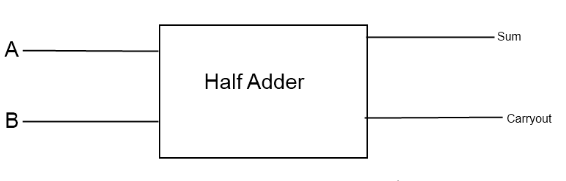
\includegraphics[scale=0.5]{half-adder-block.png}
	\captionof*{figure}{Half Adder Block Diagram}
\end{minipage}

\begin{figure}[h]
	\centering
	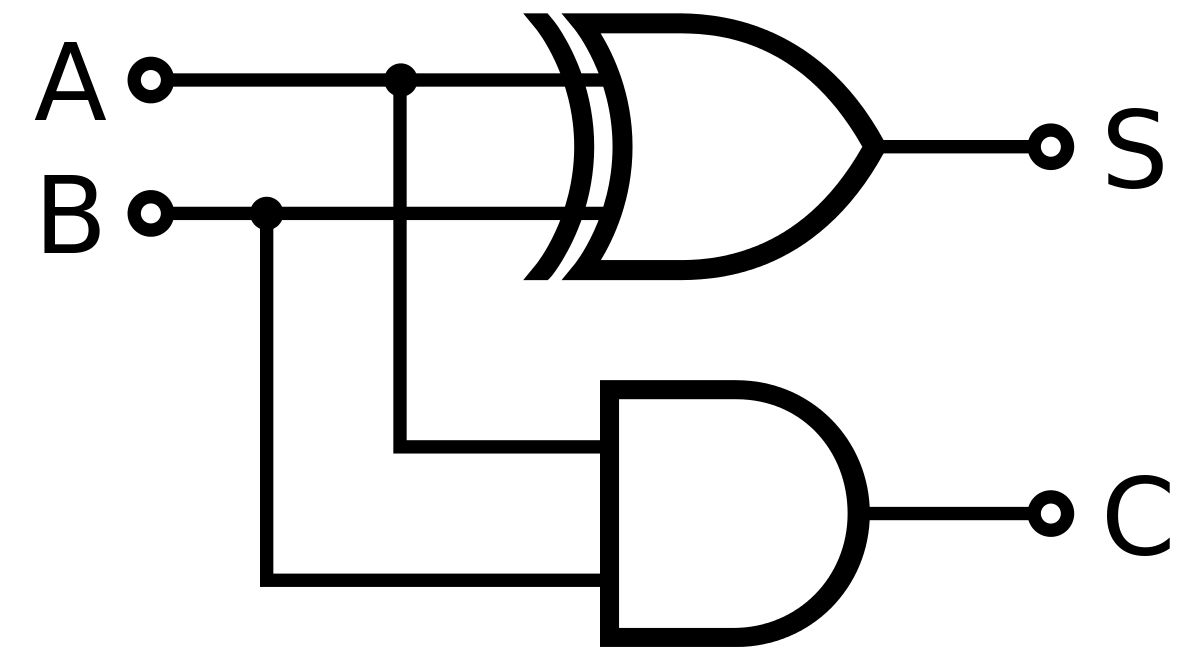
\includegraphics[scale=0.1]{half-adder-circuit.png}
	\caption{Circuit Diagram of Half Adder}
\end{figure}

\textbf{Boolean Expression}
\begin{center}
$	Sum = A \oplus B $ \\
$Carry = A . B $ \\
\end{center}
\pagebreak

\subsection{Full Adder}

Full adder is a type of adder circuit that performs 
binary addition on
its three inpus, and provides a sum and a carry value. 
Full adders are can be made by using XOR, AND and OR gates. 
A full adder can also be made by using two half adders. \\

\begin{minipage}[c]{0.4\textwidth}

	\begin{center}
	\begin{tabular}[h]{|c|c|c|c|c|}
	\hline
	A & B & C & Sum & Carry \\
	\hline
	0 & 0 & 0 & 0 & 0 \\
	0 & 0 & 1 & 1 & 0 \\
	0 & 1 & 0 & 1 & 0 \\
	0 & 1 & 1 & 0 & 1 \\
	1 & 0 & 0 & 1 & 0 \\
	1 & 0 & 1 & 0 & 1 \\
	1 & 1 & 0 & 0 & 1 \\
	1 & 1 & 1 & 1 & 1 \\
	\hline
	\end{tabular}
	\captionof{table}{Truth Table}
	\end{center}
\end{minipage}
\begin{minipage}[c]{0.55\textwidth}
	\centering
	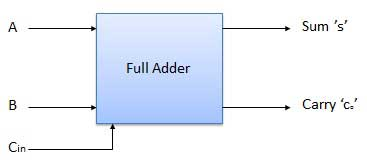
\includegraphics[scale=0.5]{full-adder-block.jpg}
	\captionof*{figure}{Full Adder Block Diagram}
\end{minipage}

\begin{figure}[h]
	\centering
	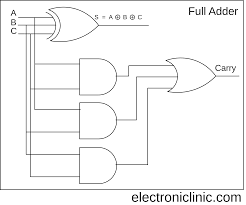
\includegraphics[scale=0.6]{full-adder-circuit.png}
	\caption{Circuit Diagram of Full Adder}
\end{figure}

\textbf{Boolean Expression}
\begin{equation}
\begin{split}
	Sum & = A'B'C + A'BC' + AB'C' + ABC \\
			& = A'(B'C + BC') + A(B'C' + BC) \\
			& = A'(B \oplus C) + A (B \oplus C)' \\
			& = A \oplus B \oplus C \\
\end{split}
\end{equation}
\begin{equation}
\begin{split}
	Carry & = A'BC + AB'C + ABC' + ABC \\
				& = BC(A + A') + A(B'C + BC') \\
				& = BC + AB'C + ABC' \\
\end{split}
\end{equation}
\pagebreak

\subsection{Half Subtractor}

A half subtractor is a combinational circuit that subracts two bits and produces their difference.
It also has an output to sepcify if a 1 has been borrowed. \\

\begin{minipage}[c]{0.45\textwidth}
	\begin{center}
	\begin{tabular}[h]{|c|c|c|c|}
	\hline
	A & B & Difference & Borrow \\
	\hline
	0 & 0 & 0 & 0 \\
	0 & 1 & 1 & 1 \\
	1 & 0 & 1 & 0 \\
	1 & 1 & 0 & 0 \\
	\hline
	\end{tabular}
	\captionof{table}{Truth Table}
	\end{center}
\end{minipage}
\begin{minipage}[c]{0.5\textwidth}
	\centering
	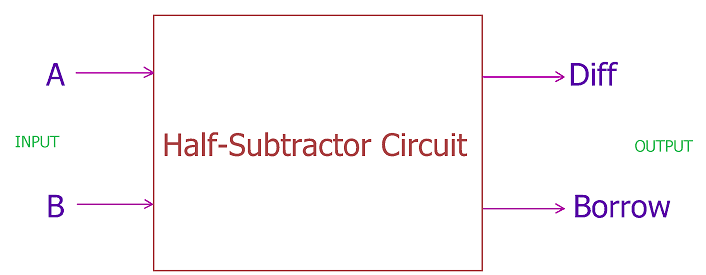
\includegraphics[scale=0.25]{half-sub-block.png}
	\captionof*{figure}{Half Subtractor Block Diagram}
\end{minipage}

\begin{figure}[h]
	\centering
	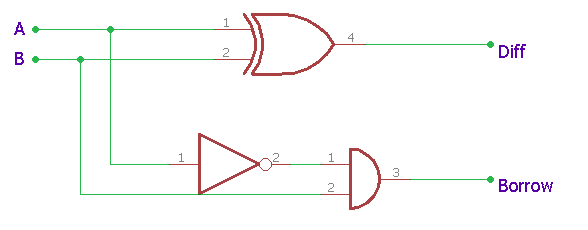
\includegraphics[scale=0.4]{half-sub-circuit.png}
	\caption{Circuit Diagram of Half Subtractor}
\end{figure}

\textbf{Boolean Expression}
\begin{center}
$	Sum = A \oplus B $ \\
$Carry = A' . B $
\end{center}
\pagebreak

\subsection{Full Subtractor}

A full subtractor is a combinational circuit that performs a subtraction between two bits, taking into account that 1 may have been borrowed
by a lower significant stage. This circuit has three inputs and two outputs.

\begin{minipage}[c]{0.4\textwidth}

	\begin{center}
	\begin{tabular}[h]{|c|c|c|c|c|}
	\hline
	A & B & $B_{in}$ & Difference & $B_{out}$\\
	\hline
	0 & 0 & 0 & 0 & 0 \\
	0 & 0 & 1 & 1 & 1 \\
	0 & 1 & 0 & 1 & 1 \\
	0 & 1 & 1 & 0 & 1 \\
	1 & 0 & 0 & 1 & 0 \\
	1 & 0 & 1 & 0 & 0 \\
	1 & 1 & 0 & 0 & 0 \\
	1 & 1 & 1 & 1 & 1 \\
	\hline
	\end{tabular}
	\captionof{table}{Truth Table}
	\end{center}
\end{minipage}
\begin{minipage}[c]{0.55\textwidth}
	\centering
	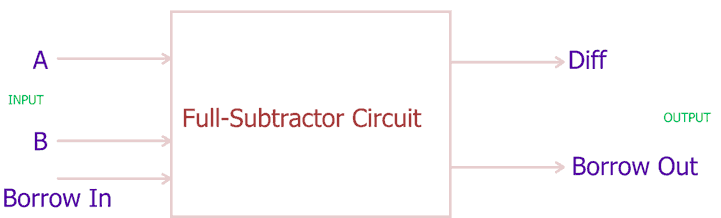
\includegraphics[scale=0.3]{full-sub-block.png}
	\captionof*{figure}{Full Subtractor Block Diagram}
\end{minipage}

\begin{figure}[h]
	\centering
	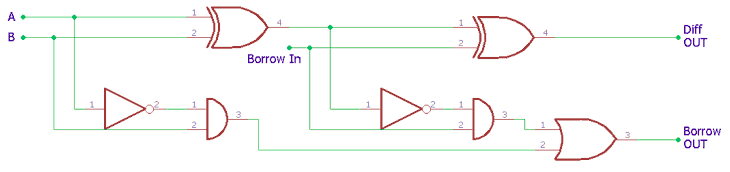
\includegraphics[scale=0.6]{full-sub-circuit.png}
	\caption{Circuit Diagram of Subtractor Adder}
\end{figure}

\textbf{Boolean Expression}
\begin{equation}
\begin{split}
	Difference&= A'B'B_{in} + A'BB_{in}' + AB'B_{in}' + ABB_{in} \\
						&= B_{in}(A'B' + AB) + B_{in}'(AB' + A'B) \\
						&= B_{in}(A \oplus B)' + B_{in}'(A \oplus B) \\
						&= B_{in} \oplus A \oplus B \\
						&= A \oplus B \oplus B_{in} \\
\end{split}
\end{equation}

\begin{equation}
\begin{split}
	B_{out} & = A'B'B_{in} + A'BB_{in}' + A'BB_{in} + ABB_{in} \\
	 				& = A'B'B_{in} + A'BB_{in}' + A'BB_{in} + A'BB_{in} + A'BB_{in} + ABB_{in} \\
					& = A'B_{in} (B + B') + A'B (B_{in} + B_{in}') + BB_{in}(A + A') \\
					& = A'B_{in} + A'B + BB_{in} \\
\end{split}
\end{equation}
\pagebreak

\subsection{Full adder using Half Adders}
Full adder can be constructed by using half adders. It requires two full adders and a Or gate. \\
\textbf{Boolean Expression}

\begin{equation}
\begin{split}
	Sum &= A\oplus B \oplus C \\
\end{split}
\end{equation}
\begin{equation}
\begin{split}
	Carry &= A'BC + AB'C + ABC' + ABC \\
				&= C(A'B + AB') + AB(C' + C) \\
				&= C(A\oplus B) + AB \\
\end{split}
\end{equation}

\begin{figure}[h]
	\centering
	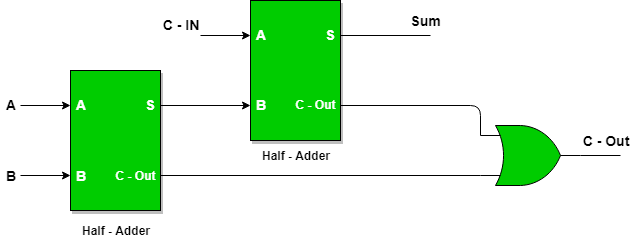
\includegraphics[scale=0.6]{half-adder-from-full-block.png}
	\caption{Block Diagram of Full Adder from Half Adders}
\end{figure}
\begin{figure}[h]
	\centering
	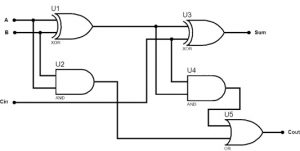
\includegraphics[scale=1]{full-adder-from-half-circuit.jpg}
	\caption{Circuit Diagram of Full Adder from half adders}
\end{figure}

\pagebreak
\subsection{Full Subtractor using Half Subtractor}
Full subtractor can be constructed by using half subtractors. 
\textbf{Boolean Expression}

\begin{equation}
	Sum = A\oplus B \oplus C \\
\end{equation}
\begin{equation}
\begin{split}
	Carry &= A'B'B_{in} + A'BB_{in} + A'BB_{in}' + ABB_{in} \\
				&= A'B(B_{in} + B_{in}') + B_{in}(A'B' + AB) \\
				& = A'B + C(A \oplus B)' \\
\end{split}
\end{equation}

\begin{figure}[h]
	\centering
	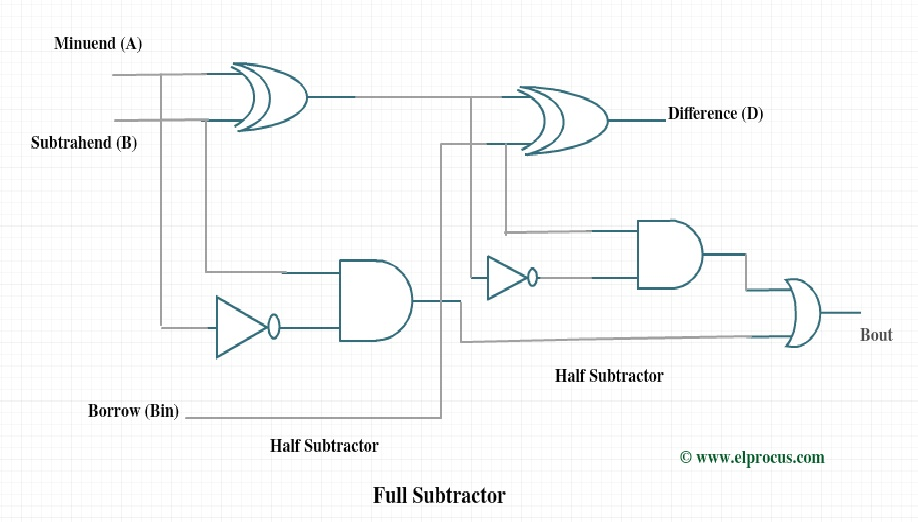
\includegraphics[scale=0.6]{full-sub-from-half-sub-circuit.jpg}
	\caption{Circuit Diagram of Full subtractor from Half Subtractor}
\end{figure}

\pagebreak

\subsection{Realization of half adder and half subtractor in a single circuit}
If we introduce a new input called switch or control state which chooses if the given two inputs will be added or subracted. We can Realize
a half adder and a half subtractor in a single circuit. We can make it so that, When S=0, addition occours and when S=1, subtraction occours.

\begin{equation}
	Sum/Difference = A \oplus B \\
\end{equation}

\begin{equation}
\begin{split}
	Borrow/Carry &= C'AB + CA'B) \\
							 &= B(C'A + CA') \\
							 &= B(C \oplus A) \\
\end{split}
\end{equation}

\begin{center}
	\begin{tabular}[h]{|c|c|c|c|c|}
	\hline
	S & A & B & Difference/Sum & Borrow/Carry \\
	\hline
	0 & 0 & 0 & 0 & 0 \\
	0 & 0 & 1 & 1 & 0 \\
	0 & 1 & 0 & 1 & 0 \\
	0 & 1 & 1 & 0 & 1 \\
	1 & 0 & 0 & 0 & 0 \\
	1 & 0 & 1 & 1 & 1 \\
	1 & 1 & 0 & 1 & 0 \\
	1 & 1 & 1 & 0 & 0 \\
	\hline
	\end{tabular}
	\captionof{table}{Truth Table}
\end{center}

\pagebreak
\subsection{Realization of full adder and full subtractor in a single circuit}
If we introduce a new input called switch or control state which chooses if the given two inputs will be added or subracted. We can Realize
a full adder and a full subtractor in a single circuit. We can make it so that, When S=0, addition occours and when S=1, subtraction occours.
\begin{equation}
\begin{split}
	Sum/Difference &= AB'C + A'B'C + ABC + A'BC' \\
			& = A'(B'C + BC') + A(B'C' + BC) \\
			& = A'(B \oplus C) + A (B \oplus C)' \\
			& = A \oplus B \oplus C \\
\end{split}
\end{equation}
\begin{equation}
\begin{split}
	Carry/Borrow &= BC + S'AC + S'AB + SA'C + SA'B \\
							 &= BC + S'AC + SA'C + S'AB + SA'B \\
							 &= BC + C(S'A + SA') +(S'A + SA') \\
							 &= BC + C(A \oplus S) + B(S \oplus A) \\
							 &= BC + (A\oplus B)(B+C) \\
\end{split}
\end{equation}

\begin{center}
	\begin{tabular}[h]{|c|c|c|c|c|c|}
	\hline
	S & A & B & C & Difference/Sum & Borrow/Carry \\
	\hline
	0 & 0 & 0 & 0 & 0 & 0 \\
	0 & 0 & 0 & 1 & 1 & 0 \\
	0 & 0 & 1 & 0 & 1 & 0 \\
	0 & 0 & 1 & 1 & 0 & 1 \\
	0 & 1 & 0 & 0 & 1 & 0 \\
	0 & 1 & 0 & 1 & 0 & 1 \\
	0 & 1 & 1 & 0 & 0 & 1 \\
	0 & 1 & 1 & 1 & 1 & 1 \\
	1 & 0 & 0 & 0 & 0 & 0 \\
	1 & 0 & 0 & 1 & 1 & 1 \\
	1 & 0 & 1 & 0 & 1 & 1 \\
	1 & 0 & 1 & 1 & 0 & 1 \\
	1 & 1 & 0 & 0 & 1 & 0 \\
	1 & 1 & 0 & 1 & 0 & 0 \\
	1 & 1 & 1 & 0 & 0 & 0 \\
	1 & 1 & 1 & 1 & 1 & 1 \\
	\hline
	\end{tabular}
	\captionof{table}{Truth Table}
\end{center}
\pagebreak

\pagebreak
\section{Lab}
\section{Half Adder}
The following half adder circuit was made in proteus
\begin{figure}[h]
	\centering
	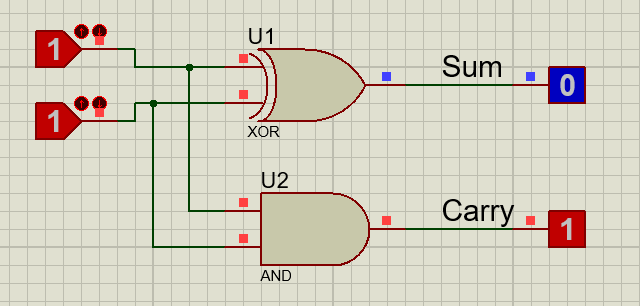
\includegraphics[scale=0.6]{half-adder.png}
	\caption{Half Adder circuit}
\end{figure}
\begin{center}
\begin{tabular}[h]{|c|c|c|c|}
	\hline
	A & B & Sum & Carry \\
	\hline
	0 & 0 & 0 & 0 \\
	0 & 1 & 1 & 0 \\
	1 & 0 & 1 & 0 \\
	1 & 1 & 0 & 1 \\
	\hline
	\end{tabular}
	\captionof{table}{Truth Table}
\end{center}


\subsection{Full Adder}
Full adder Circuit was simulated in proteus and truth table was verified.
\begin{figure}[h]
	\centering
	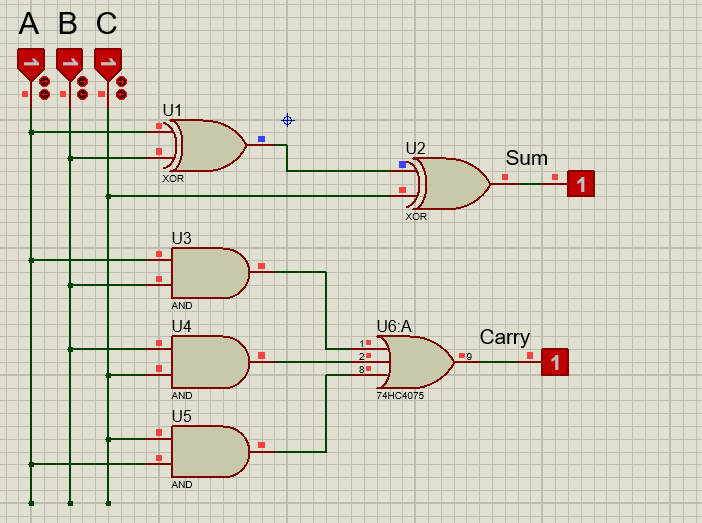
\includegraphics[scale=0.6]{full-adder.png}
	\caption{full adder circuit}
\end{figure}
	\begin{center}
	\begin{tabular}[h]{|c|c|c|c|c|}
	\hline
	A & B & C & Sum & Carry \\
	\hline
	0 & 0 & 0 & 0 & 0 \\
	0 & 0 & 1 & 1 & 0 \\
	0 & 1 & 0 & 1 & 0 \\
	0 & 1 & 1 & 0 & 1 \\
	1 & 0 & 0 & 1 & 0 \\
	1 & 0 & 1 & 0 & 1 \\
	1 & 1 & 0 & 0 & 1 \\
	1 & 1 & 1 & 1 & 1 \\
	\hline
	\end{tabular}
	\captionof{table}{Truth Table}
	\end{center}
\begin{figure}[h]
	\centering
	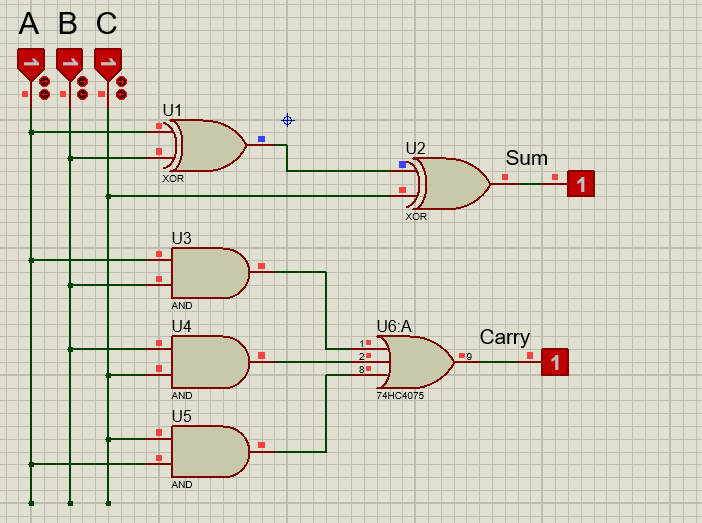
\includegraphics[scale=0.6]{full-adder.png}
	\caption{Full adder from half adders}
\end{figure}
\pagebreak

\subsection{Half Subtractor}
Half Subtractor Circuit was built, and simulated in proteus and truth table was obtained.
	\begin{center}
	\begin{tabular}[h]{|c|c|c|c|}
	\hline
	A & B & Difference & Borrow \\
	\hline
	0 & 0 & 0 & 0 \\
	0 & 1 & 1 & 1 \\
	1 & 0 & 1 & 0 \\
	1 & 1 & 0 & 0 \\
	\hline
	\end{tabular}
	\captionof{table}{Truth Table}
	\end{center}
\begin{figure}[h]
	\centering
	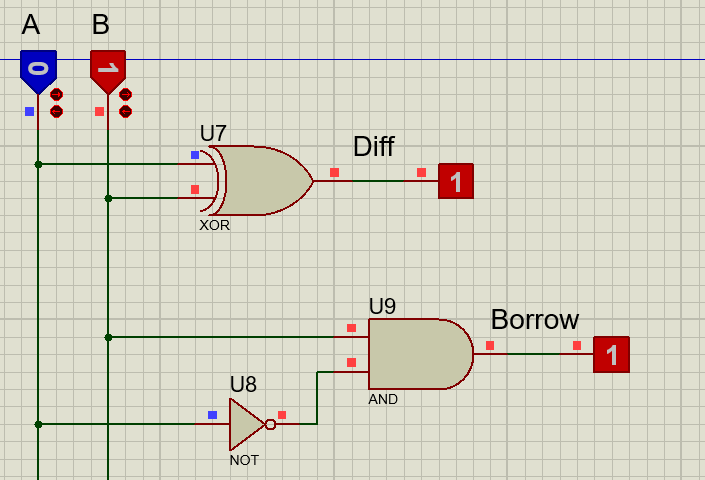
\includegraphics[scale=0.4]{half-sub.png}
	\caption{Half Subtractor}
\end{figure}
\pagebreak
\subsection{Full Subtractor}
Half Subtractor Circuit was built, and simulated in proteus and truth table was obtained.
\begin{figure}[h]
	\centering
	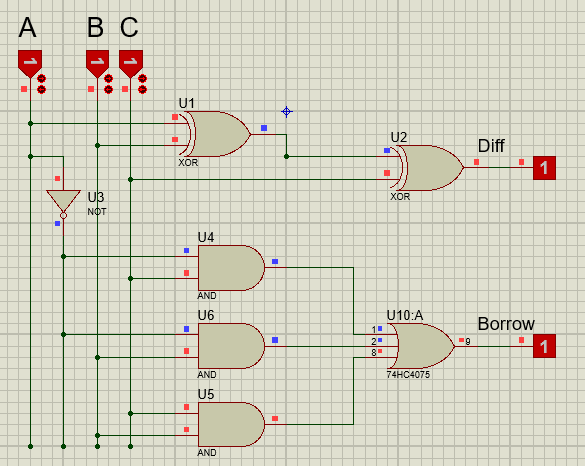
\includegraphics[scale=0.6]{full-sub.png}
	\caption{Full Subtractor}
\end{figure}

	\begin{center}
	\begin{tabular}[h]{|c|c|c|c|c|}
	\hline
	A & B & $B_{in}$ & Difference & $B_{out}$\\
	\hline
	0 & 0 & 0 & 0 & 0 \\
	0 & 0 & 1 & 1 & 1 \\
	0 & 1 & 0 & 1 & 1 \\
	0 & 1 & 1 & 0 & 1 \\
	1 & 0 & 0 & 1 & 0 \\
	1 & 0 & 1 & 0 & 0 \\
	1 & 1 & 0 & 0 & 0 \\
	1 & 1 & 1 & 1 & 1 \\
	\hline
	\end{tabular}
	\captionof{table}{Truth Table}
	\end{center}

\pagebreak

\subsection{Realization of half adder and half subtractor in a single circuit}
If we introduce a new input called switch or control state which chooses if the given two inputs will be added or subracted. We can Realize
a half adder and a half subtractor in a single circuit. We can make it so that, When S=0, addition occours and when S=1, subtraction occours.

\begin{equation}
	Sum/Difference = A \oplus B \\
\end{equation}

\begin{equation}
	Carry/Borrow = B(S \oplus A) \\
\end{equation}

\begin{figure}[h]
	\centering
	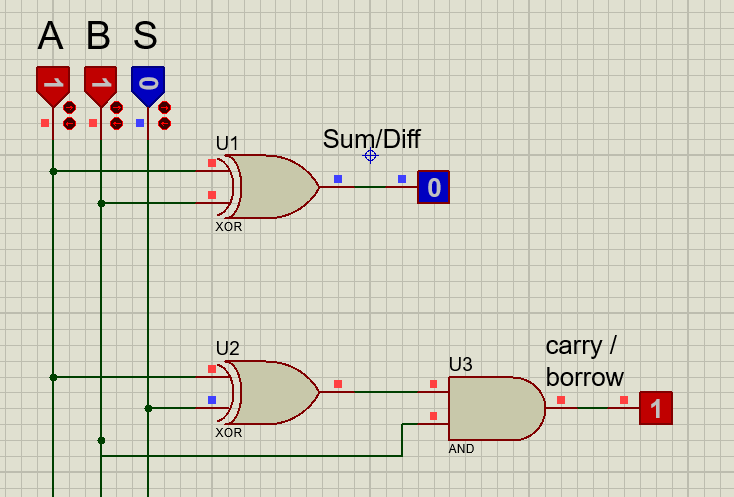
\includegraphics[scale=0.6]{half-adder-sub.png}
	\caption{Half adder and Half subtractor in a single circuit}
\end{figure}
\begin{center}
	\begin{tabular}[h]{|c|c|c|c|c|}
	\hline
	S & A & B & Difference/Sum & Borrow/Carry \\
	\hline
	0 & 0 & 0 & 0 & 0 \\
	0 & 0 & 1 & 1 & 0 \\
	0 & 1 & 0 & 1 & 0 \\
	0 & 1 & 1 & 0 & 1 \\
	1 & 0 & 0 & 0 & 0 \\
	1 & 0 & 1 & 1 & 1 \\
	1 & 1 & 0 & 1 & 0 \\
	1 & 1 & 1 & 0 & 0 \\
	\hline
	\end{tabular}
	\captionof{table}{Truth Table}
\end{center}
\pagebreak

\subsection{Realization of full adder and full subtractor in a single circuit}
If we introduce a new input called switch or control state which chooses if the given two inputs will be added or subracted. We can Realize
a full adder and a full subtractor in a single circuit. We can make it so that, When S=0, addition occours and when S=1, subtraction occours.

\begin{equation}
	Sum/Difference = A \oplus B \oplus C \\
\end{equation}

\begin{equation}
	Carry/Borrow = BC + (A \oplus S).(B+C) \\
\end{equation}

\begin{figure}[h]
	\centering
	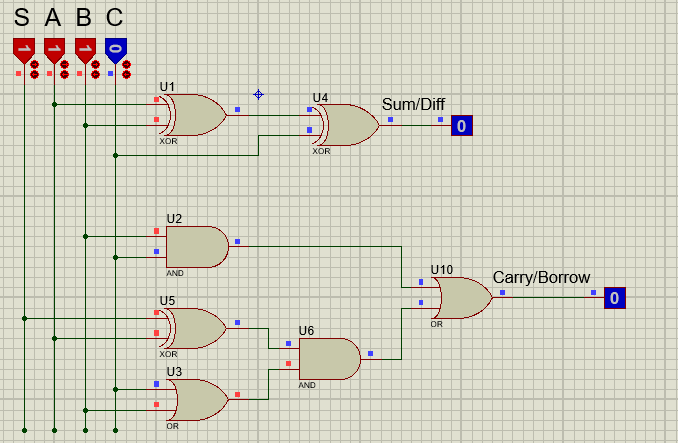
\includegraphics[scale=0.6]{full-adder-sub.png}
	\caption{Full adder and Full subtractor in a single circuit}
\end{figure}
\begin{center}
	\begin{tabular}[h]{|c|c|c|c|c|c|}
	\hline
	S & A & B & C & Difference/Sum & Borrow/Carry \\
	\hline
	0 & 0 & 0 & 0 & 0 & 0 \\
	0 & 0 & 0 & 1 & 1 & 0 \\
	0 & 0 & 1 & 0 & 1 & 0 \\
	0 & 0 & 1 & 1 & 0 & 1 \\
	0 & 1 & 0 & 0 & 1 & 0 \\
	0 & 1 & 0 & 1 & 0 & 1 \\
	0 & 1 & 1 & 0 & 0 & 1 \\
	0 & 1 & 1 & 1 & 1 & 1 \\
	1 & 0 & 0 & 0 & 0 & 0 \\
	1 & 0 & 0 & 1 & 1 & 1 \\
	1 & 0 & 1 & 0 & 1 & 1 \\
	1 & 0 & 1 & 1 & 0 & 1 \\
	1 & 1 & 0 & 0 & 1 & 0 \\
	1 & 1 & 0 & 1 & 0 & 0 \\
	1 & 1 & 1 & 0 & 0 & 0 \\
	1 & 1 & 1 & 1 & 1 & 1 \\
	\hline
	\end{tabular}
	\captionof{table}{Truth Table}
\end{center}
\pagebreak

\section{Discussion}
Various digital circuits were constructed in the practical their truth tables wre obtained. 
The truth table of the circuits and Kmap was used to obtain a boolean expression for the circuit. With this their circuits were constructed.
We got a better understanding the Combinational logic circuits. We were able to construct half adder, half subtractor, full adder, full subtractor circuits.
We also learned that full adder circuit can be constructed using 2 half adders. Similarly a full subtractor circuit can be constructed using 2 half subtractors.
We were also able to construct half adder and half subrractor in a single circuit, and similarly full andder and full subtractor in a single circuit.
This was possible with the help of a switch(S) signal. The circuit would perform addition when S=0 and subtraction when S=1.
\section{Conclusion}
Thus, a through understanding of various combinational logic circuits was obtained. Kmap was used to obtain the boolean expresstion for
half adder, half subtractor, full adder, full subtractor, half adder and half subtractor in single circuit, full adder and full subtractor 
in single circuit. These circuits were constructed and their behavour was deeply studied.

\end{document}

